\documentclass[14pt]{article}
\textwidth=13cm
\usepackage[utf8]{inputenc}
\usepackage[spanish]{babel}
\usepackage{fancyhdr}
\usepackage[pdftex]{hyperref}
\usepackage{pythonhighlight}
\usepackage[colorinlistoftodos, textwidth=4cm, shadow]{todonotes}
\RequirePackage{ifpdf} % ¿latex o pdflatex?
% Configuración de las imágenes
\ifpdf
        \usepackage[pdftex]{graphicx}  % Inclusión de imágenes
	                \DeclareGraphicsExtensions{.pdf,.png,.jpg}
\else
        \usepackage{graphicx} % Inclusión de imágenes
                        \DeclareGraphicsExtensions{.eps}
\fi
\graphicspath{ {.} } % Ruta respecto al fichero tex principal dónde se buscan imágenes

\renewcommand{\thefootnote}{\Roman{footnote}}
\hypersetup{colorlinks=true,linkcolor=black,citecolor=black}

%%%%%scabecera
\pagestyle{fancy} % seleccionamos un estilo
\lhead{UNPSJB } % texto izquierda de la cabecera
%\chead{TEXTO} % texto centro de la cabecera
\chead{Propuesta de Tesina de Licenciatura en Informática}% 
\includegraphics[width=2cm]{./unpsjb.png}} % número de página a la derecha
%\lfoot{TEXTO} % texto izquierda del pie
\rhead{
\includegraphics[scale = 0.025]{Imagenes/unpsjb.jpg}} % imagen centro del pie
%\rfoot{TEXTO} % texto derecha del pie
\renewcommand{\headrulewidth}{0.4pt} % grosor de la línea de la cabecera
\renewcommand{\footrulewidth}{0.4pt} % grosor de la línea del pie

\begin{document}

%%Caratula
\maketitle
\begin{center}

\begin{large}
  \title{\bf {Procesamiento de imágenes: Segmentacion y Medición del grosor de Vasos Sanguineos de la Retina}\\[1.5cm]
\end{large}
\date{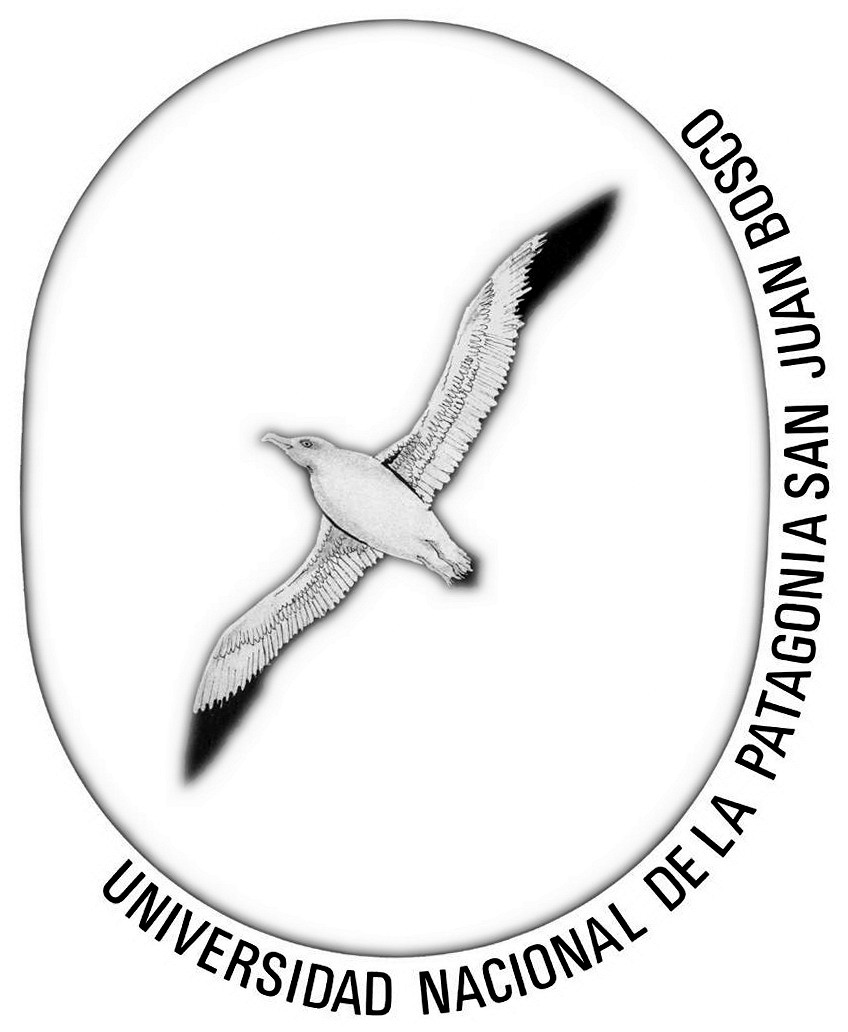
\includegraphics[scale = 0.2]{Imagenes/unpsjb1.jpg}\\[1.5cm]
\end{center}
\\
\author{Autor: Marcos Litterio\\[1cm] Tutor: Gloria Bianchi } 
%\\[1.5cm] Diciembre 2012 - UNPSJB }




%%Indice
\newpage

\tableofcontents

\newpage

\section{Palabras Clave}
\begin{enumerate}
	\item Inteligencia Artificial.
	\item Procesamiento de Imágenes.
	\item Retina.
	\item Vasos Sanguíneos.

\end{enumerate}

\section{Propuesta}
La segmentación y medición del grosor de los vasos sanguíneos de la retina es una tarea compleja y engorrosa para lograr por el humano, debido a las variaciones de colores en las imágenes, las cuales no son fácilmente perceptibles para el ojo humano. Estas variaciones deben ser segmentadas  y medidas de forma manual por un experto en el tema ,y así poder reflejar la red de los vasos sanguíneos en la retina.\\%[0.5cm] 
Tanto la medición como la segmentación pueden definirse en forma manual o en forma automática, por medio de un programa de computación.\\%[0.5cm] 



\begin{figure}[h]
	\begin{center}
		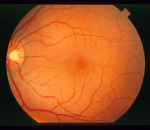
\includegraphics[scale=0.5]{./Imagenes/Retina.png}
		\caption{Imagen completa de la retina.}
	\end{center}
\end{figure} 



\begin{figure}[h]
	\begin{center}
		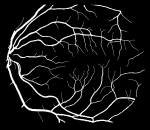
\includegraphics[scale=.5]{./Imagenes/Retinasegmentada.png}
		\caption{Imagen segmentada de la retina.}
	\end{center}
\end{figure} 


Esta tesina pone el foco en una mejora del método tradicional de segmentacion de la retina a estudiar por parte del oftalmólogo,
quien mediante sus conocimientos determina la red de vasos sanguíneos que posee la retina.\\[0.5cm]
El objetivo es automatizar estos pasos vía aplicaciones de la visión artificial, tales como segmentacion y 
detección de bordes,  como se puede observar en trabajos previos realizados por ~\cite{Gambini2006},  entre otros.\\[0.5cm]
Luego, realizar las mediciones del grosor de los vasos sanguíneos, lo cúal falicitaria la detección de cúales de ellos estan dañados y/o engrosados. Permitiendo de esta forma, indicarle al experto cúal es la situación actual de la retina\\[0.5cm]
Por último, se le brindará un resultado aproximado de la situación en la que se encuentra la retina. Para lo que utilizarán metodos que aplican inteligencia artificial.
Estos resultados, pueden darle un marco de referncia al profesional con el cúal podrá observar, por ejemplo, si una determinada retina presenta lesiones referentes a la patología conocida como \textit{retinopatia diabetica\footnote{La retinopatía diabética es una complicación ocular de la diabetes que está causada por el deterioro de los vasos sanguíneos que irrigan la retina. El daño de los vasos sanguíneos de la retina puede tener como resultado que estos sufran una fuga de fluido o sangre. Si la enfermedad avanza se forman nuevos vasos sanguíneos y prolifera el tejido fibroso en la retina, lo que tiene como consecuencia que la visión se deteriore, pues la imagen enviada al cerebro se hace borrosa.}}. Siendo de gran importancia la dectección temprana de esta enfermedad ya que no presenta (en principio) sintomas, ni dolor; esta patología es la primera causa de ceguera prevenible en adultos.





\section{Motivaciones}


\begin{enumerate}
	
	\item Incrementar mis conocimientos en el área de Procesamientos de Imágenes.
	\item Incrementar mis conocimientos en el área de Patologias Oftalmológicas.
	\item Incrementar mis conocimientos en el área de Inteligencia Artificial.
	\item Realizar un aporte al proceso de análisis de Imágenes de Retina.
	\item Concluir con mis estudios universitarios.
\end{enumerate}






\section{Objetivos}
\subsection{Primarios}
\begin{enumerate}
	\item Desarrollar una base para actuales y futuros trabajos en la segmentación y medición de imágenes oftalmológicas, particularmente imágenes de retina.\\[0.3cm]
        Para lograr este objetivo se prevé:
	\item Diseñar e implementar un software para el procesamiento de imágenes.
\end{enumerate}
Esta tesina se centrará en la segmentacion de imágenes, en particular de Retinas, lo cual daria una base para realizar procesamientos de imágenes similares, como lo podria ser el estudio del glaucoma.\\
\subsection{Secundarios}
\begin{enumerate}
	\item Investigar sobre Segmentación de Imágenes y sus aplicaciones en el ámbito de la Oftalmología.
	\item Investigar sobre teoría base y tecnologías de procesamiento de imágenes, como lo son: \emph{OpenCV}, \emph{Scipy \& Numpy}.
	\item Adquirir conocimientos sobre patologias relacionadas con la retina ocular, \emph{retinopatia diabetica} en particular. 
	\item Dar una noción y posible aplicación de IA, como soporte al análisis de la patología en cuestión.
\end{enumerate}


\section{Contexto Actual}


El procesado digital de imágenes aporta una ayuda inestimable al procesado de imágenes médicas, tanto en la automatización de procesos tediosos como en el apoyo a la decisión. Entre las imágenes oftalmológicas utilizadas en la actualidad por los profesionales del área se encuentran las angiografías, las imágenes de fondo de ojo o, más recientemente, el OCT. Las cuales, en su mayoria, se procesan manualmente por los profesionales del área, ocupando tiempo en tareas que pueden automatizarse.\\[0.5cm] Concretamente, el análisis de imágenes oftalmológicas permite la detección de las estructuras oculares, la medición automática de características y la detección de anomalías.[investigacionTIC]\\[0.5cm]
Ademas, hoy en día se encuetran en desarrollo proyectos relacionados al procesamiento de imágenes oftalmológicas referentes a la retina, como lo son  SIRIUS: Estudio de la Microcirculación Retiniana y SEDAAM: Detección Automática del Área Macular.

\subsection{SIRIUS}

'' El objetivo de este proyecto es el desarrollo de una aplicación web para la gestión centralizada de pacientes que incorpore una herramienta para el cálculo automático del índice arterio venoso a partir de imágenes de fondo de ojo siguiendo los protocolos establecidos en la literatura médica. A partir de una retinografía en color, la aplicación aborda la detección automática del disco óptico y traza un conjunto de circunferencias concéntricas a dicha estructura. A continuación, se extraen los segmentos de vaso que intersecan las circunferencias de interés y se mide su calibre. Además, loss segmentos de vaso se clasifican en arteria o vena según su intensidad de color, al igual que los expertos médicos. Por último, se realiza el cálculo del índice arteriovenoso de acuerdo a distintos métodos matemáticos.\\

La aplicación web permitirá monitorizar el estado de los pacientes y, además, proporcionará un entorno centralizado que posibilitará la realización de estudios médicos en los que intervengan distintos centros hospitalarios.   '' \cite{Sirius}

AGREGAR IMAGEN


\subsection{SEDAAM}
'' Este proyecto aborda la tarea de desarrollar una herramienta automática que permita extraer la mácula de forma automática a partir de retinografías para su posterior análisis.\\

El proceso de localización de la mácula se basa en estudios sobre la forma y disposición de las estructuras oculares. En primer lugar, se analiza el árbol arterio-venoso vascular y se determinan cuales son los vasos principales (vasos más gruesos) que aparecen en la retina. A continuación, dichos vasos principales se ajustan a un modelo polinómico y se determina el área de interés para la localización del disco óptico. Una vez localizado y segmentado el disco óptico, se ajustan los vasos principales y el disco óptico a un modelo parabólico. Este modelo permite obtener una zona de interés para la localización de la mácula. Por último, se extrae la mácula mediante usando filtros de correlación. '' \cite{Sedaam}

AGREGAR IMAGEN






\section{Resultados Esperados}

Se espera obtener un software que permita la automatización del proceseso de Segmetanción y Medición de Imágenes de la Retina, obteniendo como resultado: imagenes segmentadas de calidad de los vasos sanguineos, información referente al análisis de dicha imagen (Medicion de vasos sanguineos).


\section{Plan de Trabajo}


\begin{figure}[h]
	\begin{center}
		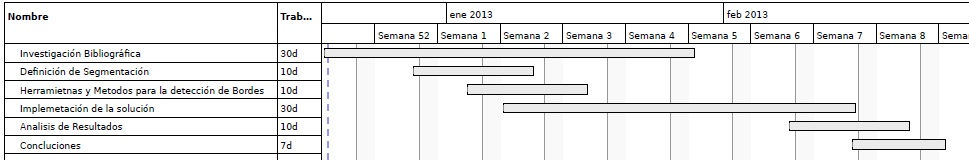
\includegraphics[scale=.5]{./Imagenes/Gantt.jpg}
		\caption{Diagrama de Gantt.}
	\end{center}
\end{figure} 



\begin{enumerate}
	\item Investigación bibliográfica.
		\begin{enumerate}
			\item Patologías Oculares (Retina): diferentes patologías, sintomas y diagnóstico.
			\item Procesamiento de imágenes: conceptos, transformaciones, segmentación, detección de bordes, etc., y tecnologías.
		\end{enumerate}
	\item Definición de segmentación, herramientas y metodos.
	\item Herramientas y metodos para la detección de bordes.
	\item Implementación de la solución.
    \item Análisis de los resultados.
	\item Conclusiones.
\end{enumerate}


\newpage
\begin{thebibliography}{1}
 	 \bibitem[Gambini 2006]{Gambini2006} Modelos de Segmentación basados en Regiones y Contornos Activos aplicados a Imágenes de Radar de Apertura Sintética. M. J. Gambini, 2006.
 	 \bibitem[Centro de investigación TIC]{investigacionTIC} \url{ http://citic-research.org/area_tecnologica/8}
 	 \bibitem[José Vicente Manjón Herrera 2006]{JVManjonHerrera2006}Segmentación Robusta de Imágenes de RM cerebral. José Vicente Manjón Herrera, 2006
	\bibitem[Cote, Hart, Goldbaum, Kube and Nelson]{CHGKN} Classification of Blood Vessels in Ocular Fundus Images. B. Cote, W. Hart, M. Goldbaum, P. Kube and M. Nelson, 1994
	\bibitem[Alvarez 2006]{Alvarez2006}Retinopatia Diabetica. Dr. Rodrigo Alvarez N., 2006
	\bibitem[Delrieux and Katz 2003]{DelrieuxKatz2003}  “Image Segmentation Through Automatic Fractal Dimension Classification”, C. Delrieux and R. Katz, 2003.
	\bibitem[Walter, Klein, Massin and Erginay 2002]{WKME2002} A contribution of image processing to de diagnosis of diabetic retinopathy – Detection of exidates in color fundus images of the human retinaT. Walter, J. Klein, P. Massin, A. Erginay, Oct. 2002.
	\bibitem[SEDAAM]{Sedaam} Detección Automática del Área Macular. Centro de investigación TIC, 2010 -2011 \url{ http://citic-research.org/actividad/proyectos/7}
	\bibitem[SIRIUS]{Sirius}Estudio de la Microcirculación Retiniana. Centro de investigación TIC, 2009 -2011 \url{ http://citic-research.org/actividad/proyectos/6}

\end{thebibliography}
\end{document}

